\section{Acoustic modeling}\label{sec:acoustic_modeling}
The first step in the DNN-HMM methodology for SI is speaker acoustic modeling, which has been approached with a historically appreciated technique: GMM-HMM (Gaussian-Mixture Model-Hidden Markov Model).

Other acoustic modeling approaches include segmental models \cite{am:segmental}, maximum entropy models~\cite{am:entropy}, and (hidden) conditional random fields \cite{am:randomfields}.

Before diving into acoustic modeling for DNN-HMM, let's introduce the statistical concepts GMM-HMM is based on.

\subsection{GMM}

A Gaussian Mixture Model (GMM) is a parametric probability density distribution represented by a weighted sum of $M$ multivariate Gaussian densities, as originally proposed by Zolfaghari and Robinson \cite{c10}.
\\Each $n$-variate Gaussian component $\mathcal{N}\left(x \mid \mu_{k}, \Sigma_{k}\right)$ resembles the distribution of a cluster in the dataset, and can be defined by two parameters:

\begin{description}
    \item[Mean vector:] $\mu_k = [\mu_{k, 1}, \mu_{k, 2}, ..., \mu_{k, n}]$, correspondig to the $k$-th cluster's centroid $\frac{1}{|G_k|}\sum_{x \in G_k} x$;
    
    \item[Covariance matrix:] $\Sigma_k = ||\sigma^{(k)}_{i, j}||_{n \times n} $ such that $\sigma^{(k)}_{i, j} = Cov(X_{k, i}, X_{k, j})$ is the covariance between the $i$-th and the $j$-th feature of the samples belonging to the $k$-cluster $G_k$;
\end{description}
and thus it can be expressed as:
$$
\mathcal{N}\left(x \mid \mu_{k}, \Sigma_{k}\right)=\frac{1}{(2 \pi)^{\frac{D}{2}}\left|\Sigma_{k}\right|^{\frac{1}{2}}} e^{-\frac{1}{2}\left(x-\mu_{k}\right)^{T} \Sigma_{k}^{-1}\left(x-\mu_{k}\right)}
$$
That being said, a GMM is defined as a weighted combination of $M$ $n$-variate Gaussian densities, called components:

$$
P(x \mid \lambda)=\sum_{k=1}^{M} w_{k} \, \mathcal{N}\left(x \mid \mu_{k}, \Sigma_{k}\right),
$$
where:
$$
\sum_{k=1}^{M} w_{k}=1
$$
In GMM training, dataset clusters (and thus parameters of Gaussian components) are initially computed using a clustering algorithm (e.g. $k$-means), and then adjusted using an E-M algorithm (such as MLE \cite{mlegmm} or MAP \cite{mapgmm}), which works even if the clusters overlap with each other, since this type of algorithm uses the probability of an instance $x$ to belong to a cluster $G_j$, rather than the distance from its centroid.
\\Concerning the component weights $w_1, w_2, ..., w_M$, they are initialized randomly and then also tuned with the E-M algorithm alongside the mean vectors and covariance matrices.

Based on the structure and constraints of covariance matrices, GMMs can be divided in some different groups:

\begin{description}
    \item[Full:] each Gaussian component has its own general covariance matrix, thus the generated clusters can adopt any position/shape;
    
    \item[Tied:] each Gaussian component has the same general covariance matrix, hence the generated clusters can have any position (means), but must have the same shape;
    
    \item[Diagonal:] each Gaussian component has its own diagonal covariance matrix (i.e. the only non-zero entries are variances $\sigma^{(k)}_{i, i} = Var(X_{k, i})$), thus each cluster can have any shape, but their contour axes must be oriented along the coordinate axes;
    
    \item[Tied diagonal:] each Gaussian component has the same diagonal covariance matrix, hence each cluster must have the same shape and their contour axes must be oriented along the coordinate axes;
    
    \item[Spherical:] identical to the diagonal case, but the variances within the same covariance matrix are equal (i.e. $\sigma^{(k)}_{i, i} = \sigma^{(k)}_{j, j}, \forall i, j \in \{1, 2, ..., n\}$), thus each cluster must have a circular shape (although not necessarily the same circular shape), and their contour axes be oriented along the coordinate axes.
\end{description}

\subsection{HMM}

Hidden Markov Model (HMM) is a statistical modeling technique with an underlying couple of stochastic processes, an hidden (i.e. not observable) one, and an observable one. 

The hidden stochastic process is represented by finite set of possible states, called \textbf{hidden state space} $S = \{s_1, s_2, ..., s_K\}$, transitioning to each other overtime with fixed probabilities, generating a sequence of states $q_1, q_2, ..., q_T$. \\
The main assumption on which HMM are built is that the probability of transiting into a state $s_i$ at the time $t$ depends solely on the previous state $q_{t-1}$ (this is also called Markov Hypothesis \cite{markovbook}), hence:

$$P(q_t = s_i \, | \, q_1, q_2, ..., q_{t-1}) = P(q_t = s_i \, | \, q_{t-1})$$
this makes possible to collect these probabilities \textbf{transition matrix}:

$$
A = 
\begin{bmatrix}
    t_{1,1} & t_{1,2} & \dots  & t_{1, K} \\
    t_{2, 1} & t_{2, 2} & \dots  & t_{2, K} \\
    \vdots & \vdots & \ddots & \vdots \\
    t_{K, 1} & t_{K, 2} & \dots  & t_{K, K}
\end{bmatrix}, \text{ where:}
$$

$$t_{i, j} = P(q_t = s_i \, | \, q_{t-1} = s_j);$$
this transition matrix can be viewed as one of the three fundamental parameters that define an HMM. Based on the structure of the transition matrix, several HMM \textit{topologies} are defined (as seen in Figure \vref{fig:topologies_ergodic}, 
\vref{fig:topologies_left_to_right},
\vref{fig:topologies_left_to_right_cyclic},
\vref{fig:topologies_bidirectional}):

\begin{description}
    \item[Ergodic:] there is no 0 probability in the transition matrix, $t_{i, j} > 0, \forall i,j \in \{1,2, ..., K\}$, so each state can be reached from each state with a non-zero probability; 
    
    \item[Left-to-right:] there exists a topological order between the states $q_1, q_2, ..., q_K$ such that for every non-zero transition $t_{i, j} > 0 \implies i < j$; 
    
    \item[Left-to-right cyclic:] there exists an ordering between the states $q_1, q_2, ..., q_K$ such that for every non-zero transition $t_{i, j} > 0 \implies i \leq j$ (there can also be self-loops);
    
    \item[Bidirectional:] the HMM transitions can be split in two sets $A, B$ such that each transition $t_{i, j} > 0 \in A \implies i \leq j$ and $t_{i, j} > 0 \in B \implies i \geq j$.
\end{description}

\begin{figure}[!ht]
    \begin{center}
    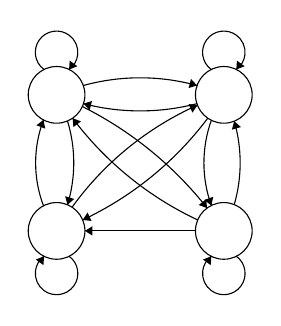
\begin{tikzpicture}[scale=0.12]
    \tikzstyle{every node}+=[inner sep=0pt]
    \draw [black] (3.2,-7.2) circle (3);
    \draw [black] (20.9,-7.2) circle (3);
    \draw [black] (3.2,-21.6) circle (3);
    \draw [black] (20.9,-21.6) circle (3);
    \draw [black] (6.03,-6.212) arc (105.44309:74.55691:22.607);
    \fill [black] (18.07,-6.21) -- (17.43,-5.52) -- (17.17,-6.48);
    \draw [black] (1.877,-4.52) arc (234:-54:2.25);
    \fill [black] (4.52,-4.52) -- (5.4,-4.17) -- (4.59,-3.58);
    \draw [black] (19.577,-4.52) arc (234:-54:2.25);
    \fill [black] (22.22,-4.52) -- (23.1,-4.17) -- (22.29,-3.58);
    \draw [black] (4.523,-24.28) arc (54:-234:2.25);
    \fill [black] (1.88,-24.28) -- (1,-24.63) -- (1.81,-25.22);
    \draw [black] (4.355,-9.963) arc (17.01386:-17.01386:15.162);
    \fill [black] (4.35,-18.84) -- (5.07,-18.22) -- (4.11,-17.93);
    \draw [black] (22.223,-24.28) arc (54:-234:2.25);
    \fill [black] (19.58,-24.28) -- (18.7,-24.63) -- (19.51,-25.22);
    \draw [black] (17.9,-21.6) -- (6.2,-21.6);
    \fill [black] (6.2,-21.6) -- (7,-22.1) -- (7,-21.1);
    \draw [black] (18.134,-20.44) arc (-115.17821:-143.08258:35.384);
    \fill [black] (4.9,-9.67) -- (4.98,-10.61) -- (5.78,-10.01);
    \draw [black] (5.932,-8.438) arc (63.42803:38.31117:39.131);
    \fill [black] (19.13,-19.18) -- (19.03,-18.24) -- (18.24,-18.86);
    \draw [black] (19.201,-9.671) arc (-36.93255:-64.80665:35.421);
    \fill [black] (5.97,-20.44) -- (6.9,-20.55) -- (6.48,-19.65);
    \draw [black] (4.842,-19.09) arc (144.19742:114.06338:32.897);
    \fill [black] (18.11,-8.3) -- (17.17,-8.17) -- (17.58,-9.08);
    \draw [black] (19.58,-18.913) arc (-160.26378:-199.73622:13.365);
    \fill [black] (19.58,-18.91) -- (19.78,-17.99) -- (18.84,-18.33);
    \draw [black] (18.051,-8.134) arc (-75.44882:-104.55118:23.886);
    \fill [black] (6.05,-8.13) -- (6.7,-8.82) -- (6.95,-7.85);
    \draw [black] (1.817,-18.946) arc (-159.19201:-200.80799:12.796);
    \fill [black] (1.82,-9.85) -- (1.07,-10.42) -- (2,-10.78);
    \draw [black] (22.003,-9.985) arc (16.17554:-16.17554:15.847);
    \fill [black] (22,-9.99) -- (21.75,-10.89) -- (22.71,-10.61);
    \end{tikzpicture}
    \end{center}
    \caption{Ergodic}
\label{fig:topologies_ergodic}
\end{figure}

\begin{figure}[!ht]
    \begin{center}
    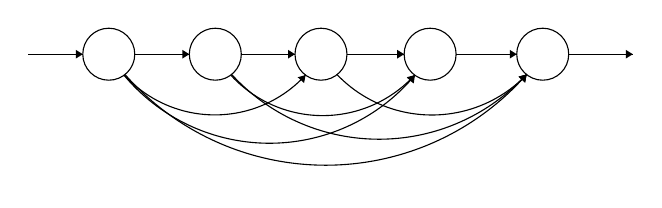
\begin{tikzpicture}[scale=0.11]
    \tikzstyle{every node}+=[inner sep=0pt]
    \draw [black] (11.5,-7.7) circle (3);
    \draw [black] (23.8,-7.7) circle (3);
    \draw [black] (36,-7.7) circle (3);
    \draw [black] (48.6,-7.7) circle (3);
    \draw [black] (61.6,-7.7) circle (3);
    \draw [black] (2.2,-7.7) -- (8.5,-7.7);
    \fill [black] (8.5,-7.7) -- (7.7,-7.2) -- (7.7,-8.2);
    \draw [black] (34.219,-10.107) arc (-42.54859:-137.45141:14.21);
    \fill [black] (34.22,-10.11) -- (33.31,-10.36) -- (34.05,-11.03);
    \draw [black] (46.84,-10.127) arc (-39.87576:-140.12424:21.878);
    \fill [black] (46.84,-10.13) -- (45.94,-10.42) -- (46.71,-11.06);
    \draw [black] (46.821,-10.108) arc (-42.43129:-137.56871:14.389);
    \fill [black] (46.82,-10.11) -- (45.91,-10.36) -- (46.65,-11.04);
    \draw [black] (59.729,-10.044) arc (-41.37756:-138.62244:30.89);
    \fill [black] (59.73,-10.04) -- (58.83,-10.31) -- (59.58,-10.97);
    \draw [black] (59.72,-10.035) arc (-42.55769:-137.44231:23.106);
    \fill [black] (59.72,-10.04) -- (58.81,-10.29) -- (59.55,-10.96);
    \draw [black] (59.748,-10.054) arc (-43.84962:-136.15038:15.181);
    \fill [black] (59.75,-10.05) -- (58.83,-10.28) -- (59.55,-10.98);
    \draw [black] (14.5,-7.7) -- (20.8,-7.7);
    \fill [black] (20.8,-7.7) -- (20,-7.2) -- (20,-8.2);
    \draw [black] (26.8,-7.7) -- (33,-7.7);
    \fill [black] (33,-7.7) -- (32.2,-7.2) -- (32.2,-8.2);
    \draw [black] (39,-7.7) -- (45.6,-7.7);
    \fill [black] (45.6,-7.7) -- (44.8,-7.2) -- (44.8,-8.2);
    \draw [black] (51.6,-7.7) -- (58.6,-7.7);
    \fill [black] (58.6,-7.7) -- (57.8,-7.2) -- (57.8,-8.2);
    \draw [black] (64.6,-7.7) -- (72,-7.7);
    \fill [black] (72,-7.7) -- (71.2,-7.2) -- (71.2,-8.2);
    \end{tikzpicture}
    \end{center}
    \caption{Left-to-right}
    \label{fig:topologies_left_to_right}
\end{figure}
\begin{figure}[!ht]
    \begin{center}
    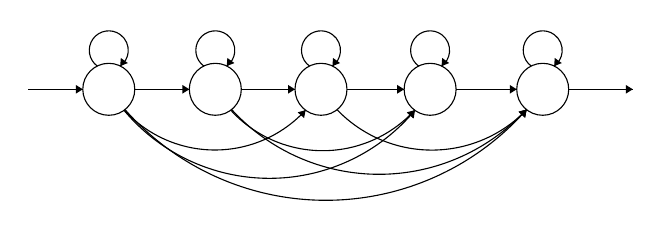
\begin{tikzpicture}[scale=0.11]
    \tikzstyle{every node}+=[inner sep=0pt]
    \draw [black] (11.5,-7.7) circle (3);
    \draw [black] (23.8,-7.7) circle (3);
    \draw [black] (36,-7.7) circle (3);
    \draw [black] (48.6,-7.7) circle (3);
    \draw [black] (61.6,-7.7) circle (3);
    \draw [black] (10.177,-5.02) arc (234:-54:2.25);
    \fill [black] (12.82,-5.02) -- (13.7,-4.67) -- (12.89,-4.08);
    \draw [black] (22.477,-5.02) arc (234:-54:2.25);
    \fill [black] (25.12,-5.02) -- (26,-4.67) -- (25.19,-4.08);
    \draw [black] (34.677,-5.02) arc (234:-54:2.25);
    \fill [black] (37.32,-5.02) -- (38.2,-4.67) -- (37.39,-4.08);
    \draw [black] (47.277,-5.02) arc (234:-54:2.25);
    \fill [black] (49.92,-5.02) -- (50.8,-4.67) -- (49.99,-4.08);
    \draw [black] (2.2,-7.7) -- (8.5,-7.7);
    \fill [black] (8.5,-7.7) -- (7.7,-7.2) -- (7.7,-8.2);
    \draw [black] (34.219,-10.107) arc (-42.54859:-137.45141:14.21);
    \fill [black] (34.22,-10.11) -- (33.31,-10.36) -- (34.05,-11.03);
    \draw [black] (46.84,-10.127) arc (-39.87576:-140.12424:21.878);
    \fill [black] (46.84,-10.13) -- (45.94,-10.42) -- (46.71,-11.06);
    \draw [black] (46.821,-10.108) arc (-42.43129:-137.56871:14.389);
    \fill [black] (46.82,-10.11) -- (45.91,-10.36) -- (46.65,-11.04);
    \draw [black] (59.729,-10.044) arc (-41.37756:-138.62244:30.89);
    \fill [black] (59.73,-10.04) -- (58.83,-10.31) -- (59.58,-10.97);
    \draw [black] (59.72,-10.035) arc (-42.55769:-137.44231:23.106);
    \fill [black] (59.72,-10.04) -- (58.81,-10.29) -- (59.55,-10.96);
    \draw [black] (59.748,-10.054) arc (-43.84962:-136.15038:15.181);
    \fill [black] (59.75,-10.05) -- (58.83,-10.28) -- (59.55,-10.98);
    \draw [black] (14.5,-7.7) -- (20.8,-7.7);
    \fill [black] (20.8,-7.7) -- (20,-7.2) -- (20,-8.2);
    \draw [black] (26.8,-7.7) -- (33,-7.7);
    \fill [black] (33,-7.7) -- (32.2,-7.2) -- (32.2,-8.2);
    \draw [black] (39,-7.7) -- (45.6,-7.7);
    \fill [black] (45.6,-7.7) -- (44.8,-7.2) -- (44.8,-8.2);
    \draw [black] (51.6,-7.7) -- (58.6,-7.7);
    \fill [black] (58.6,-7.7) -- (57.8,-7.2) -- (57.8,-8.2);
    \draw [black] (64.6,-7.7) -- (72,-7.7);
    \fill [black] (72,-7.7) -- (71.2,-7.2) -- (71.2,-8.2);
    \draw [black] (60.277,-5.02) arc (234:-54:2.25);
    \fill [black] (62.92,-5.02) -- (63.8,-4.67) -- (62.99,-4.08);
    \end{tikzpicture}
    \end{center}
    \caption{Left-to-right cyclic}
    \label{fig:topologies_left_to_right_cyclic}
\end{figure}
\begin{figure}[!ht]
    \begin{center}
    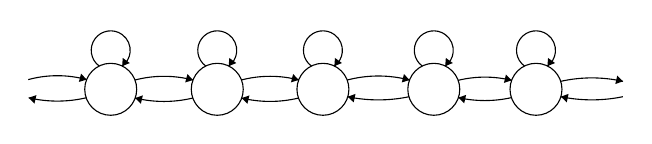
\begin{tikzpicture}[scale=0.11]
    \tikzstyle{every node}+=[inner sep=0pt]
    \draw [black] (11.5,-7.7) circle (3);
    \draw [black] (23.8,-7.7) circle (3);
    \draw [black] (36,-7.7) circle (3);
    \draw [black] (48.8,-7.7) circle (3);
    \draw [black] (60.6,-7.7) circle (3);
    \draw [black] (10.177,-5.02) arc (234:-54:2.25);
    \fill [black] (12.82,-5.02) -- (13.7,-4.67) -- (12.89,-4.08);
    \draw [black] (22.477,-5.02) arc (234:-54:2.25);
    \fill [black] (25.12,-5.02) -- (26,-4.67) -- (25.19,-4.08);
    \draw [black] (34.677,-5.02) arc (234:-54:2.25);
    \fill [black] (37.32,-5.02) -- (38.2,-4.67) -- (37.39,-4.08);
    \draw [black] (47.477,-5.02) arc (234:-54:2.25);
    \fill [black] (50.12,-5.02) -- (51,-4.67) -- (50.19,-4.08);
    \draw [black] (1.976,-6.581) arc (105.25754:74.74246:12.821);
    \fill [black] (8.72,-6.58) -- (8.08,-5.89) -- (7.82,-6.85);
    \draw [black] (14.295,-6.628) arc (104.54663:75.45337:13.357);
    \fill [black] (21,-6.63) -- (20.36,-5.94) -- (20.1,-6.91);
    \draw [black] (26.592,-6.622) arc (104.5773:75.4227:13.142);
    \fill [black] (33.21,-6.62) -- (32.56,-5.94) -- (32.31,-6.9);
    \draw [black] (38.798,-6.632) arc (104.79702:75.20298:14.105);
    \fill [black] (46,-6.63) -- (45.36,-5.94) -- (45.1,-6.91);
    \draw [black] (51.609,-6.664) arc (103.66979:76.33021:13.081);
    \fill [black] (57.79,-6.66) -- (57.13,-5.99) -- (56.9,-6.96);
    \draw [black] (63.451,-6.781) arc (102.63452:77.36548:16.452);
    \fill [black] (70.65,-6.78) -- (69.98,-6.12) -- (69.76,-7.09);
    \draw [black] (59.277,-5.02) arc (234:-54:2.25);
    \fill [black] (61.92,-5.02) -- (62.8,-4.67) -- (61.99,-4.08);
    \draw [black] (57.764,-8.662) arc (-77.38859:-102.61141:14.035);
    \fill [black] (51.64,-8.66) -- (52.31,-9.32) -- (52.53,-8.35);
    \draw [black] (45.93,-8.561) arc (-78.2626:-101.7374:17.353);
    \fill [black] (38.87,-8.56) -- (39.55,-9.21) -- (39.76,-8.23);
    \draw [black] (33.181,-8.71) arc (-76.43152:-103.56848:13.986);
    \fill [black] (26.62,-8.71) -- (27.28,-9.38) -- (27.51,-8.41);
    \draw [black] (20.98,-8.707) arc (-76.40618:-103.59382:14.169);
    \fill [black] (14.32,-8.71) -- (14.98,-9.38) -- (15.21,-8.41);
    \draw [black] (8.67,-8.679) arc (-76.81873:-103.18127:14.559);
    \fill [black] (2.03,-8.68) -- (2.7,-9.35) -- (2.92,-8.37);
    \draw [black] (70.628,-8.554) arc (-78.3068:-101.6932:17.654);
    \fill [black] (63.47,-8.55) -- (64.15,-9.21) -- (64.36,-8.23);
    \end{tikzpicture}
    \end{center}
    \caption{Bidirectional}
\label{fig:topologies_bidirectional}
\end{figure}
The second fundamental parameter of an HMM is the \textbf{prior distribution} vector, which defines the probability that a sequence of states $q_1, q_2, ..., q_T$ has of starting with each state $s_1, s_2, ..., s_K$:

$$\pi = [\pi_1, \pi_2, ..., \pi_K], \text{ where:}$$
$$\pi_i = P(q_1 = s_i), \forall i \in \{1, 2, ..., K\}.$$
The third and last parameter of HMM is the so-called \textbf{emission distribution}. As said before, an HMM has two underlying stochastic processes: an hidden and an observable one; similar to the former, the latter also produces a sequence over time, called \textit{observation sequence} $o_1, o_2, ..., o_T$.
At each time $t$, the \textbf{emission distribution} defines the probability density function (or discrete density function if the possible observation are countable) of an observation $o_t$, given the current state $s_t$:

$$e(o_t \, | \, s_t) = f_D(o_t \, | \, s_t) \text{ (continuous case) } $$

$$e(o_t \, | \, s_t) = P(o_t \, | \, s_t) \text{ (discrete case).} $$
Given a set of observations:
$$X = \{x^{(1)}, x^{(2)}, ..., x^{(m)}\}\text{, }$$
an HMM is trained with an E-M algorithm to maximize the likelihood of the observations:

$$A^*, B^*, \pi^* = \arg \max_{A, B, \pi} P(X \, | \, A, B, \pi)$$
A particularly useful application of the E-M approach to HMMs is the Viterbi algorithm, a dynamic programming algorithm originally proposed by Andrew Viterbi \cite{viterbi}, which makes possible to compute in polynomial time the most likely sequence of states, given a sequence of observations:

$$q^*_1, ..., q^*_T = \arg \max_{q_1, ..., q_T} P(q_1, ..., q_T \, | \, o_1, ..., o_T)\text{.}$$
The idea of the algorithm is to express this probability through a recurrence relationship, and then use classic dynamic programming with memoization to compute its value faster (and in polynomial time, which wouldn't be possible otherwise).
\\The recurrence relationship used to express the probability of the most likely sequence of state, given the observations $o_1, o_2, ..., o_T$ is the following:

$$V_{1, k} = P(o_1 \, | \, k) \, \pi_k, \, \forall k \in S$$
$$V_{t, k} = \max_{q \, \in \, S} P(o_t \, | \, q) \, A_{q, s_k} \, V_{t-1, q} \text{, }$$
where $A$ is the transition matrix and $\pi$ is the prior distribution. The algorithm operates as follows:

\begin{enumerate}[label=(\roman*), font=\itshape]
    \item computes the base case probabilities $V_{1, k}$ for each state $k$, storing it into a $T \times K$ matrix $V$;
    
    \item computes each remaining entry $V_{t, k}$ of the matrix according to the recurrent relationship, taking advantage of the already stored values in the matrix, and storing into another matrix $\Ptr$ the state used to compute $V_{k, t}$ (representing the most likely state to transition from, into state $s_k$ at time $t$):
    
    $$\Ptr_{t, k} = \arg \max_{q} P(o_t \, | \, q) \cdot A_{q, s_k} \cdot V_{t-1, q}$$
    
    \item computes the most likely sequence of states using the computed values in the $V$ matrix, retrieving the sequence backwards:
    
    \begin{enumerate}[label=(\alph*), font=\itshape]
        \item $q^*_T = \arg \max_q V_{T, q}$;
        \\
        \item $q^*_{t-1} = \Ptr_{t, q^*_t}$
    \end{enumerate}
\end{enumerate}



\subsection{GMM-HMM} 
Given these definitions, a GMM-HMM is a HMM where emission distribution of each state is defined by a GMM with $M$ Gaussians:

$$e(o_t \, | \, s) = P(o_t \mid \lambda)=\sum_{k=1}^{M} w_{k} \, \mathcal{N}\left(x \mid \mu_{k}, \Sigma_{k}\right),$$
Often, GMM-HMM are used to build acoustic models that represent the feature distribution of a specific class of audios, which is useful in a plenty of different tasks. In speech recognition for example, GMM-HMM acoustic models are built to represent the phoneme distribution \cite{gmmhmmspeechrecognition}, \cite{asr:dnnhmm0}, and each state corresponds to a phoneme, while in scene classification each GMM-HMM acoustic model is built to represent the audios recorded in a particular scene/context \cite{dnnhmmscene}. 

Not too differently, in SI task, which is the main subject of this study, GMM-HMM acoustic models are built to represent the audios recorded by a specific speaker. Therefore, for $p$ speakers there will be $p$ GMM-HMM models, each trained with an E-M algorithm on utterances of the corresponding speaker:

$$\HMM_1, \HMM_2, ..., \HMM_p$$
At identification time, an unknow audio $o = o_1, o_2, ..., o_T$ is scored against each GMM-HMM acoustic model using Viterbi algoritm \cite{gmmhmmspeakeridentification}, and the speaker is identified by the most likely path among all the speaker acoustic models:

$$s = \arg \max_i \Viterbi_P(o, \HMM_i) \text{, }$$
where $\Viterbi_P(o, \HMM_i)$ is the posterior probability of the most likely $\HMM_i$ state path given $o$, according to the Viterbi algorithm:

$$\Viterbi_P(o, \HMM_i) = \max_{q_1, ..., q_T} P_{i}(q_1, ..., q_T \, | \, o_1, ..., o_T)$$
This methodology has been successfully applied in multiple past studies with good results \cite{gmmhmmspeakeridentification}, alongside with the GMM-standalone acoustic modeling, which was applied to the TIMIT dataset too \cite{gmmspeakeridentification}.

As for the choice of the state number $K$ for each acoustic model, it is either chosen application domain-wise, in tasks like speech recognition where each state can represent a phoneme (e.g. triphone \cite{asr:triphone}), or can be chosen empirically through grid search methods, using instance likelihood as score.
\\The same applies to the mixture number $M$, whose optimal value can vary considerably depending on the dataset, as shown in multiple studies \cite{si:gmmhmm1}, \cite{si:gmmhmm2}, \cite{polishasr:gmmhmm}.

Finally, it is important to note that each HMM topology suits different types of tasks; in ASR, for example, letf-to-right topologies are often used, since it fits the phonetic structure of speech, which involves some phonemes before others overtime. In SI or scene classification, on the other hand, the most suitable topology turns out to be the ergodic \cite{si:dnnhmm}, \cite{dnnhmmscene}, since the structure of audio recognition patterns for these two types of task may not necessarily be ordered, as they are not related to phonemes.

\paragraph{GMM-HMM in DNN-HMM}
In DNN-HMM approach to SI, GMM-HMM acoustic models are built using feature extracted from the utterances of the training set (often MFCCs/MFCCs \& deltas \cite{si:dnnhmm}) to represent the audios recorded by each speaker, and then used with Viterbi algorithm to generate frame-level audio labels that will be later used to train the DNN model.

More specifically, for each audio $o = o_1, o_2, ..., o_T$ from the speaker $j$, where each $o_t$ is an audio frame containing some kind of feature (raw audio, power/log-scaled STFT spectrum, power/log-scaled Mel spectrum, MFCCs/ MFCCs \& deltas, LPCCs, ...), Viterbi algorithm is applied to generate the most likely state sequence (this step is sometimes also called "forced alignment" \cite{si:dnnhmm}, \cite{dnnhmmscene}):

$$q^* = q^*_1, q^*_2, ..., q^*_T = \Viterbi(o, \HMM_j) \text{, }$$
where $\Viterbi(o, \HMM_j)$ is the most likely $\HMM_j$ state path given $o$, according to the Viterbi algorithm:
$$\Viterbi(o, \HMM_j) = \arg \max_{q_1, ..., q_T} P_j(q_1, ..., q_T | o_1, ..., o_T)$$
The generated states $q^* = q^*_1, q^*_2, ..., q^*_T$ are used as frame-level labels for the audio frames $o = o_1, o_2, ..., o_T$, so that each frame $o_t$ corresponds to the state label $q^*_t$. 
\\As will be explained shortly, these labels will later be used to train the underlying DNN model used in the DNN-HMM approach.

In this study, grid search has been performed to optimize the mixture $M$ and state number $K$ of our ergodic GMM-HMM acoustic models with diagonal covariance type. Results have been varying depending on the type of features used, as shown in table \vref{tab:gmmhmmgridsearch}.

It's noteworthy that acoustic models generated using log-scaled Mel-spectrum and LPCC features were not used in later stages of the study (e.g. training of the neural network model), but were generated for comparative purposes only (although this could be subject of future studies).

\begin{footnotesize}
	\begin{table}
		\centering
		\caption{GMM-HMM grid-search Results}
		\label{tab:grid_search_results}
		\begin{tabularx}{0.5\textwidth}{Xcc}
			\toprule
			\textbf{Feature} 			& \textbf{States} & \textbf{Mixtures}    \\
			\midrule
			MFCCs \& deltas	              		& 8                      & 3         \\[0.25cm]
			LPCCs             			& 4                      & 2         \\[0.25cm]
			Log-scaled Mel Spectrum features   			& 3  					 & 2         \\ 
			\bottomrule
		\end{tabularx}
		
	\end{table}\label{tab:gmmhmmgridsearch}
	
\end{footnotesize}
